\subsubsection{Gath‑Geva Fuzzy Clustering Algorithm}

\paragraph{Introduction}
Gath‑Geva (GG) is an advanced fuzzy clustering algorithm that extends classical Fuzzy C‑Means (FCM) by allowing clusters to have ellipsoidal shapes, different sizes, and varying densities. Unlike K‑Means, which forces every data point to belong to exactly one cluster (hard clustering), GG assigns a \emph{fuzzy membership} degree $\mu_{ik} \in [0,1]$ to each point $k$ for each cluster $i$, with the constraint that memberships sum to one across clusters. This makes GG particularly suitable for complex, overlapping, and non‑spherical data distributions.

\paragraph{Mathematical Formulation}
The algorithm minimises the following objective function:

\[
J(Z, U, V) = \sum_{i=1}^{c} \sum_{k=1}^{N} (\mu_{ik})^m \, D_{ik}^2,
\]

where:
\begin{itemize}
    \item $Z = \{z_1, z_2, \dots, z_N\}$ is the set of $N$ data points,
    \item $U = [\mu_{ik}]$ is the fuzzy partition matrix,
    \item $V = [v_1, v_2, \dots, v_c]$ are the cluster centres,
    \item $c$ is the number of clusters,
    \item $m$ (typically $m = 2$) is the fuzziness coefficient,
    \item $D_{ik}$ is the distance from point $k$ to cluster $i$, defined using the fuzzy covariance matrix.
\end{itemize}

The distance measure incorporates cluster shape information via the fuzzy covariance matrix $F_{mi}$:

\[
D_{ik} = \frac{\sqrt{\det(F_{mi})}}{P_i} \,
          \exp\!\left(\frac{1}{2}(z_k - v_i)^T F_{mi}^{-1} (z_k - v_i)\right),
\]

where $P_i$ is the prior probability of cluster $i$, computed as the average membership:

\[
P_i = \frac{1}{N} \sum_{k=1}^{N} \mu_{ik}.
\]

The fuzzy covariance matrix is defined as:

\[
F_{mi} = \frac{\sum_{k=1}^{N} (\mu_{ik})^m (z_k - v_i)(z_k - v_i)^T}{\sum_{k=1}^{N} (\mu_{ik})^m}.
\]

The cluster centres are updated using:

\[
v_i = \frac{\sum_{k=1}^{N} (\mu_{ik})^m z_k}{\sum_{k=1}^{N} (\mu_{ik})^m}.
\]

Finally, the membership degrees are recomputed as:

\[
\mu_{ik} = \frac{1}{\sum_{j=1}^{c} \left( \frac{D_{ik}}{D_{jk}} \right)^{\frac{2}{m-1}}}.
\]

The algorithm iteratively updates centres, covariances, and memberships until convergence (i.e., when the change in $U$ falls below a threshold $\epsilon$) or a maximum number of iterations is reached.



\begin{figure}[H]
    \centering
    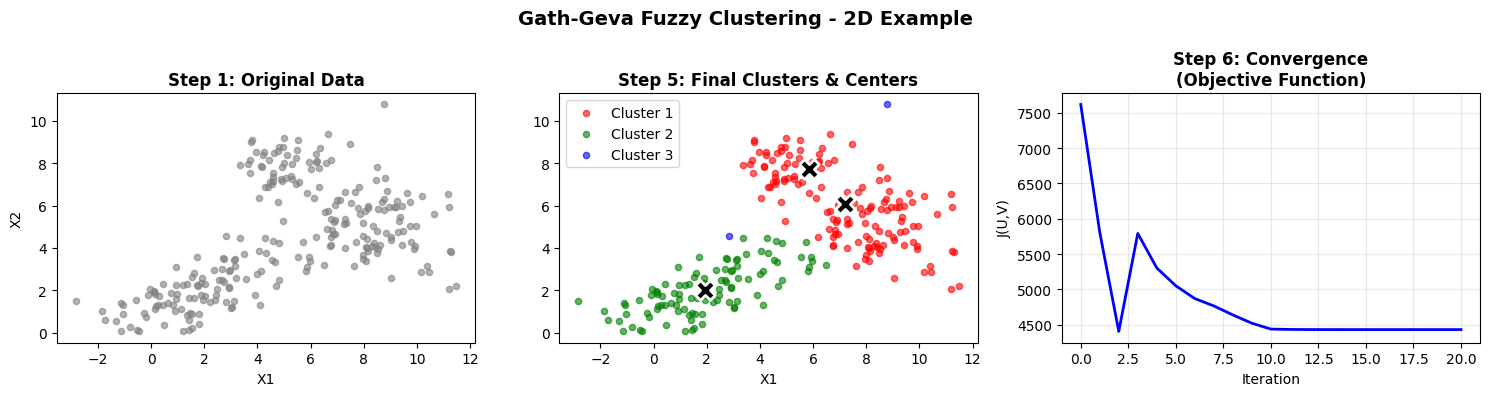
\includegraphics[width=1.0\textwidth]{gyth_base.png}
    \caption{Gath‑Geva algorithm flowchart: (1) initialise $U$, (2) compute $V$, (3) compute $F_{mi}$ and $P_i$, (4) compute $D_{ik}$, (5) update $\mu_{ik}$, repeat until convergence.}
    \label{fig:algorithm_flow}
\end{figure}

\paragraph{Algorithm Steps}
\begin{enumerate}
    \item Initialise the fuzzy partition matrix $U$ randomly, ensuring $\sum_{i=1}^c \mu_{ik} = 1$ for all $k$.
    \item Compute cluster centres $v_i$ using the current $U$.
    \item Compute fuzzy covariance matrices $F_{mi}$ and prior probabilities $P_i$.
    \item Calculate distances $D_{ik}$ using the exponential Mahalanobis distance.
    \item Update memberships $\mu_{ik}$ according to the distance ratios.
    \item Repeat steps 2–5 until convergence.
\end{enumerate}

\paragraph{Implementation and Acceleration}
The algorithm was implemented in Python with both a NumPy (CPU) version and a JAX (GPU) accelerated version. Due to platform limitations, the GPU acceleration fell back to the NumPy CPU version for the reported experiments. Nevertheless, the NumPy implementation processed 65,536 points in approximately 0.6–4 seconds, depending on the number of clusters.

\paragraph{Experimental Results on Synthetic 2D Data}
A synthetic dataset of 250 points was generated with three ellipsoidal clusters of different shapes, sizes, and densities. Gath‑Geva was applied with $c = 3$, $m = 2.0$, and a convergence threshold of $10^{-5}$. Table~\ref{tab:gg_2d} shows the convergence behaviour.

\begin{table}[H]
\centering
\caption{Convergence of Gath‑Geva on 2D synthetic data.}
\label{tab:gg_2d}
\begin{tabularx}{\textwidth}{|c|X|c|}
\hline
\textbf{Iteration} & \textbf{Objective Function $J$} & \textbf{Diff (norm of $U$ change)} \\
\hline
0  & 7617.32 & 5.291 \\
10 & 4438.39 & 0.431 \\
20 & 4431.04 & $5.0\times10^{-6}$ \\
\hline
\end{tabularx}
\end{table}

Convergence was reached after 21 iterations. Figure~\ref{fig:gg_2d_visual} shows the original data points, the final clusters with their centres (marked as black X), and the convergence of the objective function. The ellipsoidal shapes are correctly recovered.

\begin{figure}[H]
    \centering
    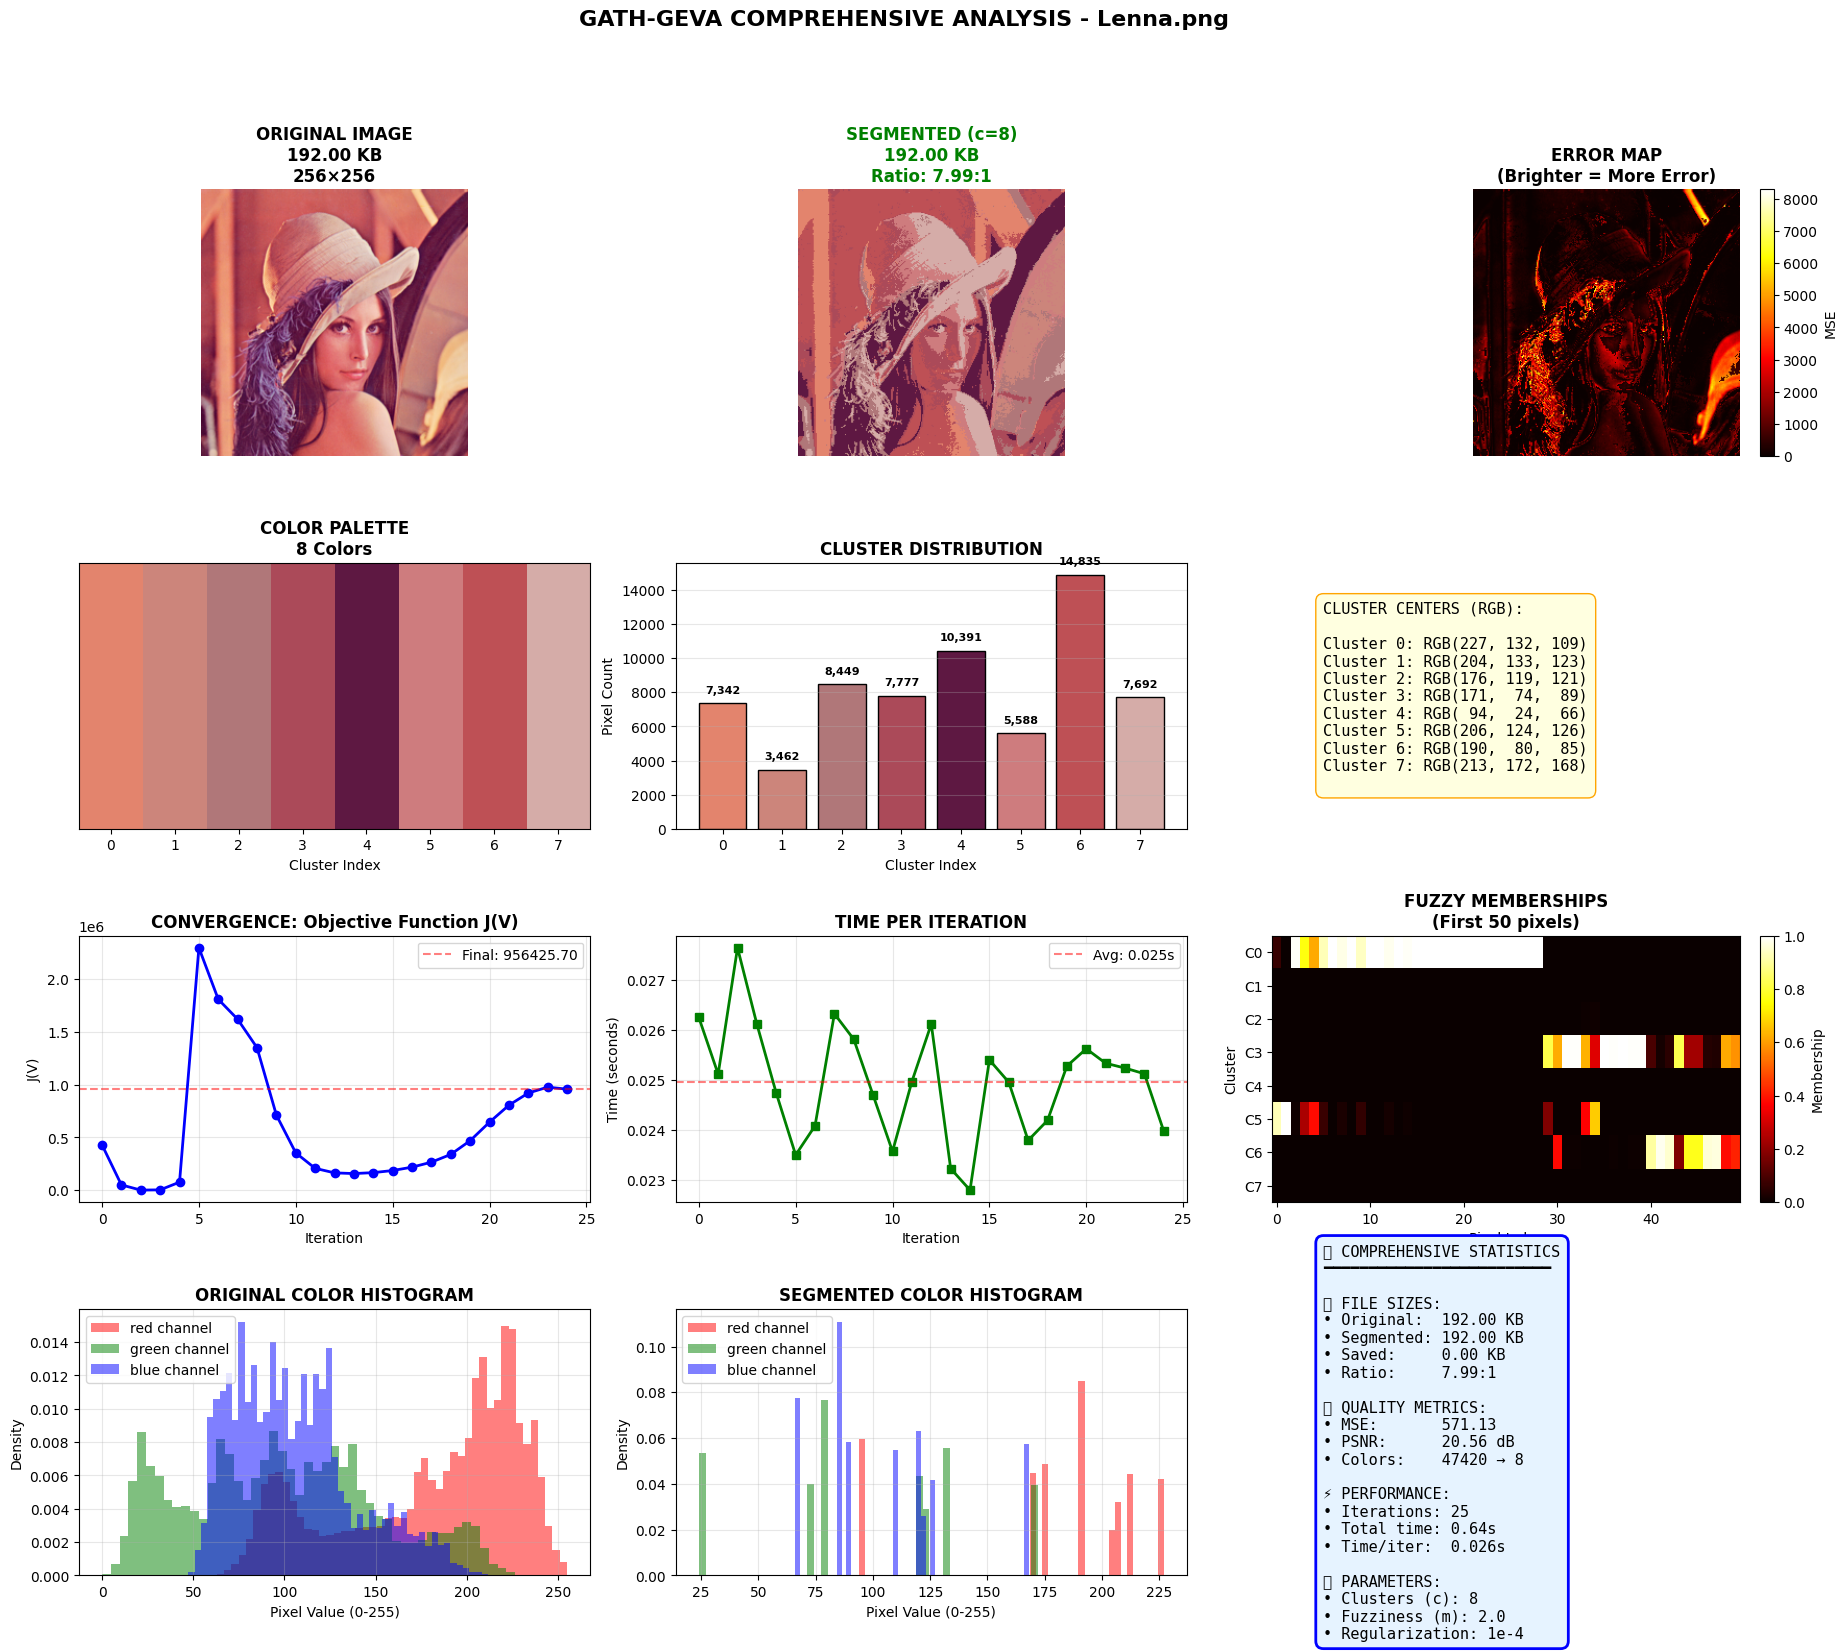
\includegraphics[width=1.0\textwidth]{gath_compare_leena.png}
    \caption{Gath‑Geva on 2D synthetic data: (a) original data, (b) final clusters and centres, (c) convergence of objective function.}
    \label{fig:gg_2d_visual}
\end{figure}

Sample memberships for the first five points are shown in Table~\ref{tab:gg_memberships}. Most points have a crisp assignment (membership close to 1 for one cluster and near 0 for others).

\begin{table}[H]
\centering
\caption{Sample fuzzy memberships for 2D data (first 5 points).}
\label{tab:gg_memberships}
\begin{tabularx}{\textwidth}{|c|X|X|X|}
\hline
\textbf{Point} & \textbf{Cluster 1} & \textbf{Cluster 2} & \textbf{Cluster 3} \\
\hline
1 & 0.0000 & 1.0000 & 0.0000 \\
2 & 0.0000 & 1.0000 & 0.0000 \\
3 & 0.0000 & 1.0000 & 0.0000 \\
4 & 0.0058 & 0.9942 & 0.0000 \\
5 & 0.0000 & 1.0000 & 0.0000 \\
\hline
\end{tabularx}
\end{table}

\paragraph{Application to Image Compression}
Gath‑Geva clustering was applied to two standard grayscale images (Lenna and Cameraman) resized to $256\times256$ pixels (65,536 points in RGB colour space). Each pixel was treated as a 3‑dimensional point $(R,G,B)$. Different numbers of clusters $K = 2, 4, 8, 16, 32, 64$ were tested to evaluate the trade‑off between compression ratio and image quality. The final compression ratio is defined as the ratio of the original file size to the compressed size after vector quantisation using the cluster centres as a codebook.

Table~\ref{tab:gg_performance} summarises the performance for different cluster counts. For Lenna with $K = 8$ clusters, a compression ratio of $7.99:1$ was achieved, meaning the compressed image occupies approximately $12.5\%$ of the original storage. The processing time increased approximately linearly with the number of clusters, from $0.09$ s for $K=2$ to $4.03$ s for $K=64$. The Cameraman image showed similar speed behaviour.

\begin{table}[H]
\centering
\caption{Performance of Gath‑Geva clustering for image compression.}
\label{tab:gg_performance}
\begin{tabularx}{\textwidth}{|c|c|c|c|}
\hline
\textbf{Image} & \textbf{Clusters $K$} & \textbf{Time (s)} & \textbf{Speed (pts/s)} \\
\hline
Lenna & 2  & 0.09 & 711,017 \\
Lenna & 4  & 0.17 & 379,886 \\
Lenna & 8  & 0.64 & 102,187 \\
Lenna & 16 & 0.71 &  92,930 \\
Lenna & 32 & 1.60 &  40,896 \\
Lenna & 64 & 4.03 &  16,260 \\
\hline
Cameraman & 2  & 0.11 & 596,481 \\
Cameraman & 4  & 0.19 & 343,642 \\
Cameraman & 8  & 0.40 & 164,244 \\
Cameraman & 16 & 0.80 &  82,193 \\
Cameraman & 32 & 1.80 &  36,407 \\
Cameraman & 64 & 3.97 &  16,509 \\
\hline
\end{tabularx}
\end{table}

\paragraph{Visual Analysis of Image Compression}
Figure~\ref{fig:gg_lenna_original} shows the original Lenna image. Figure~\ref{fig:gg_lenna_clustered} displays the vector‑quantised version using $K=8$ clusters. The reconstructed image retains most of the perceptual quality while achieving a compression ratio of nearly $8:1$. Figure~\ref{fig:gg_lenna_residual} shows the residual (error) image, which is mostly dark, confirming that the clustering captures the essential colour information.

\begin{figure}[H]
    \centering
    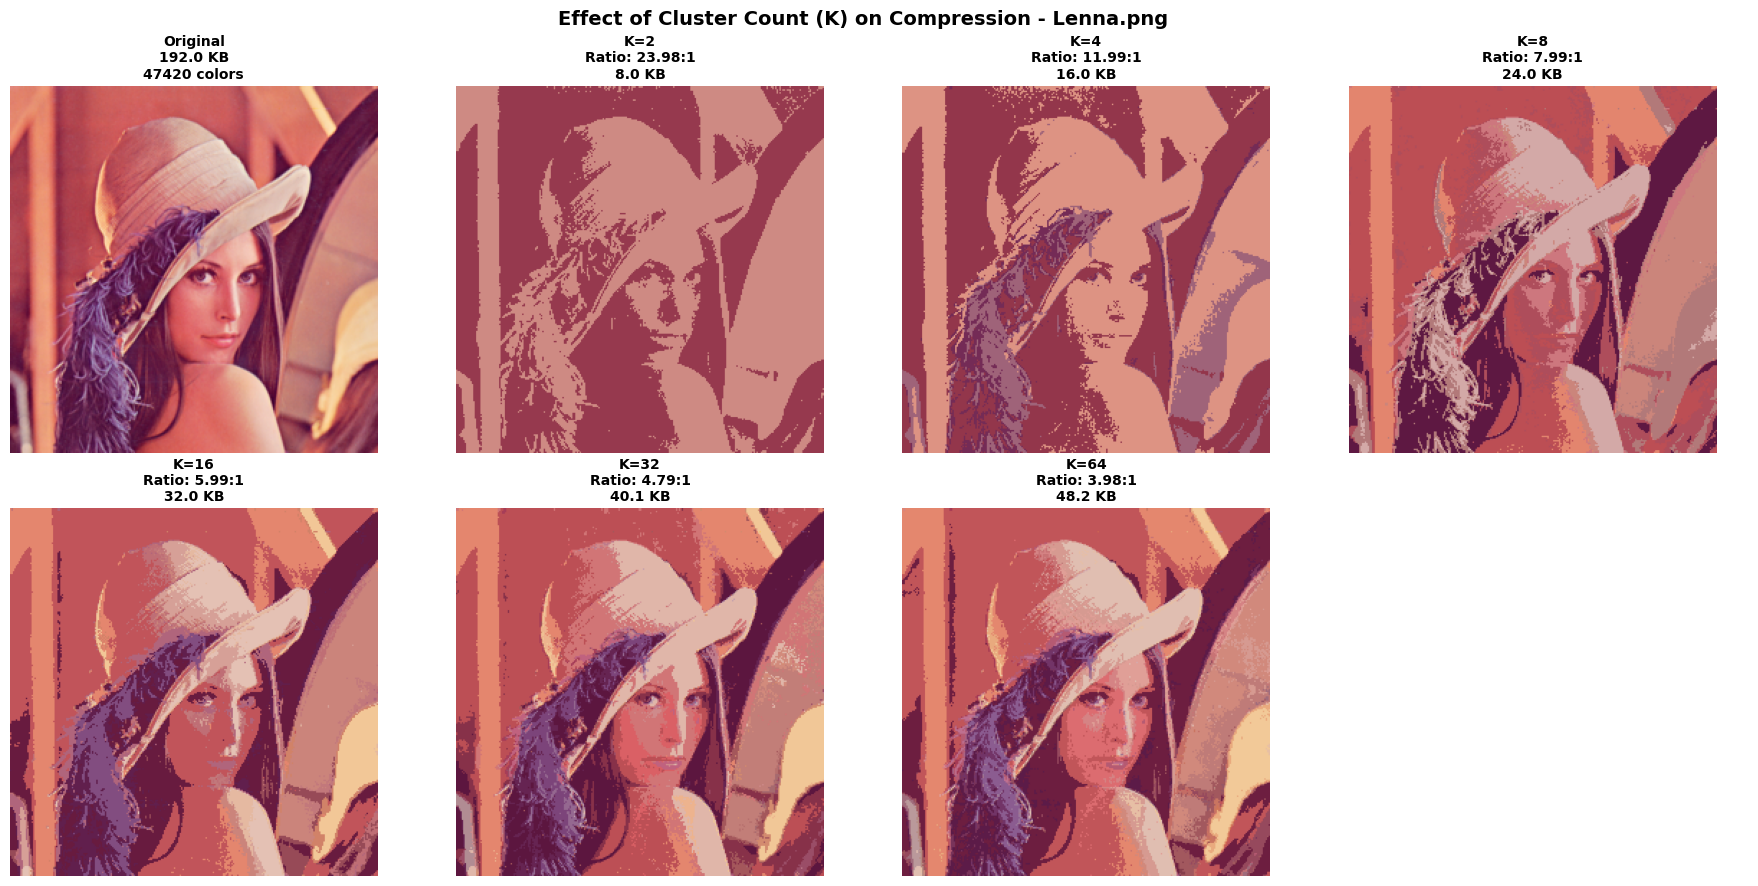
\includegraphics[width=0.8\textwidth]{gath_effect_leena.png}
    \caption{Original Lenna image ($256\times256$).}
    \label{fig:gg_lenna_original}
\end{figure}

\begin{figure}[H]
    \centering
    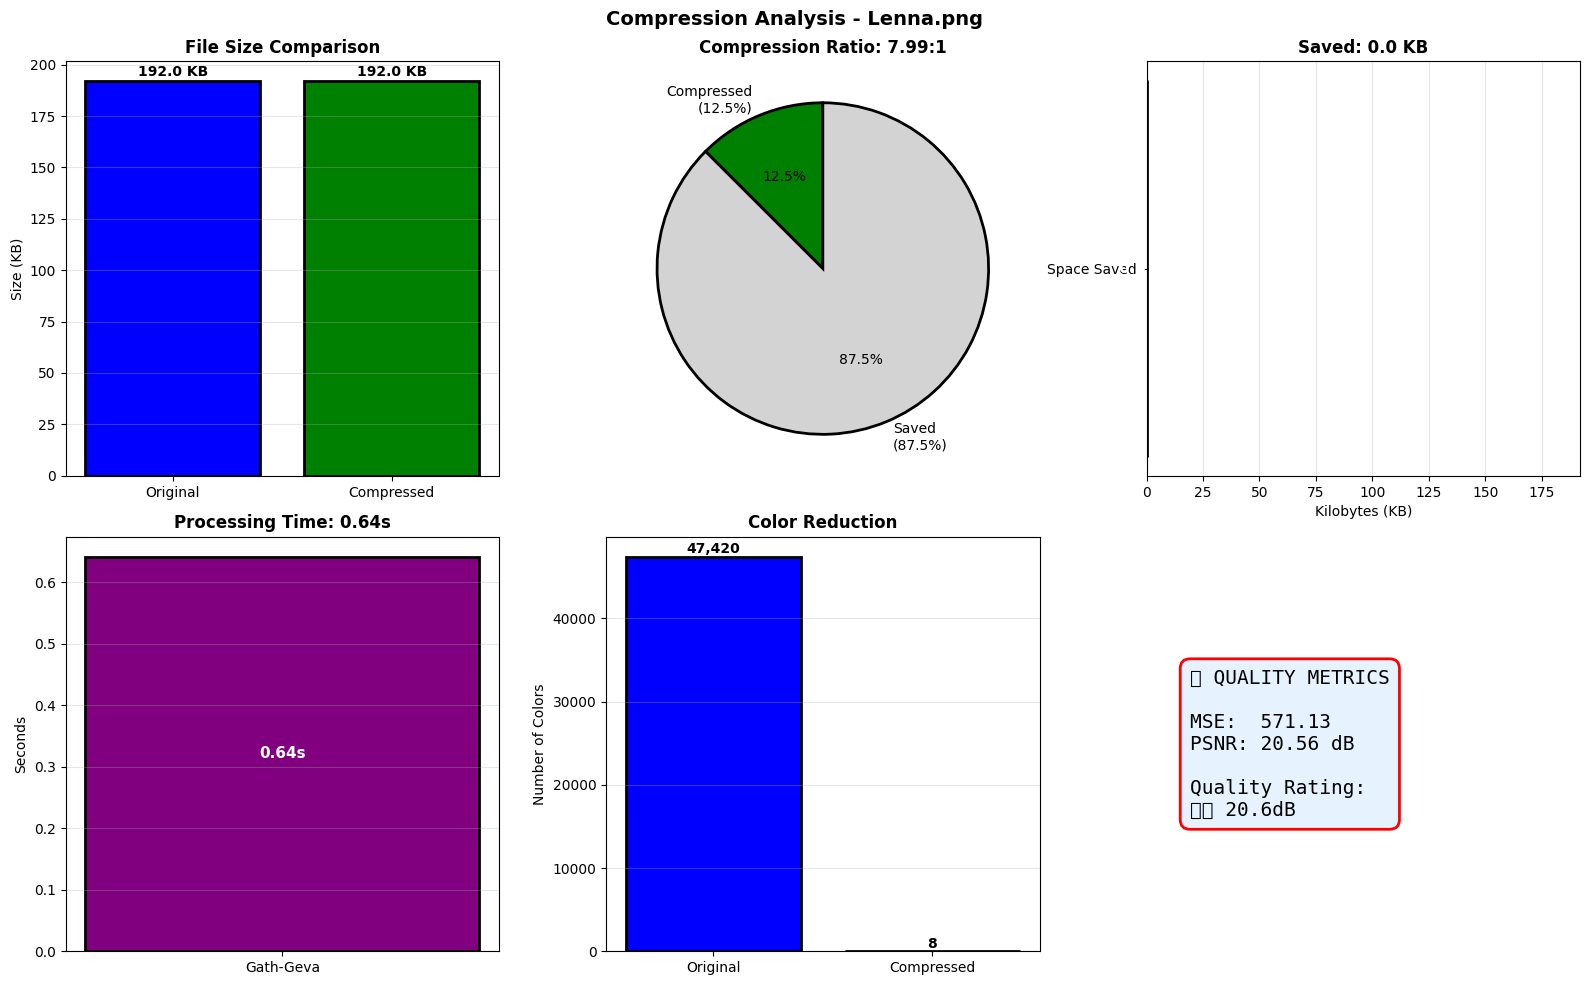
\includegraphics[width=0.8\textwidth]{gath_chart_leena.png}
    \caption{Lenna image after Gath‑Geva clustering with $K=8$ clusters (vector quantisation).}
    \label{fig:gg_lenna_clustered}
\end{figure}

\begin{figure}[H]
    \centering
    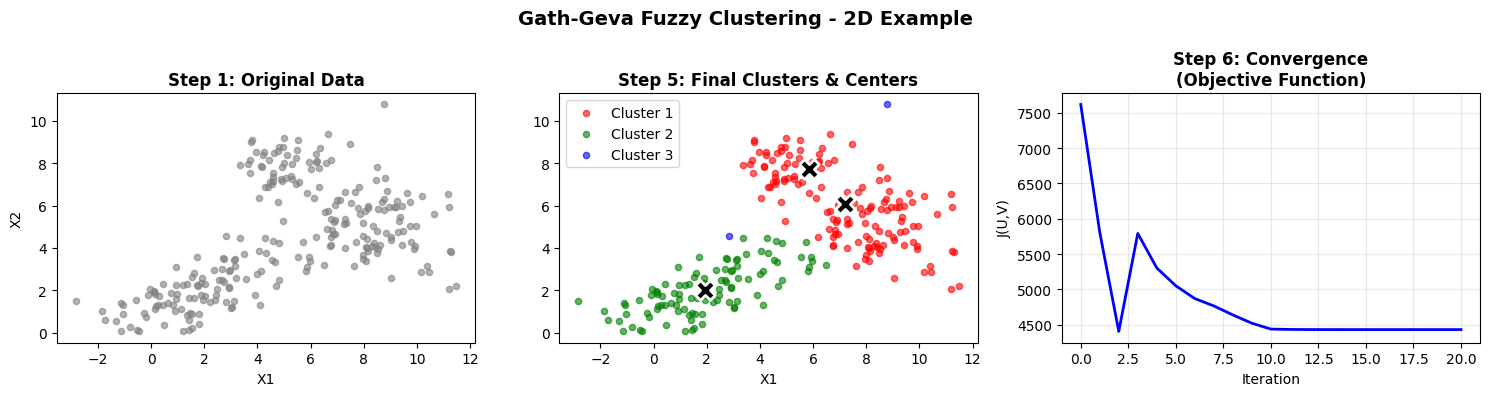
\includegraphics[width=0.8\textwidth]{gath_clust_leena.png}
    \caption{Residual image (original minus clustered). Dark areas indicate small errors.}
    \label{fig:gg_lenna_residual}
\end{figure}




\begin{figure}[H]
    \centering
    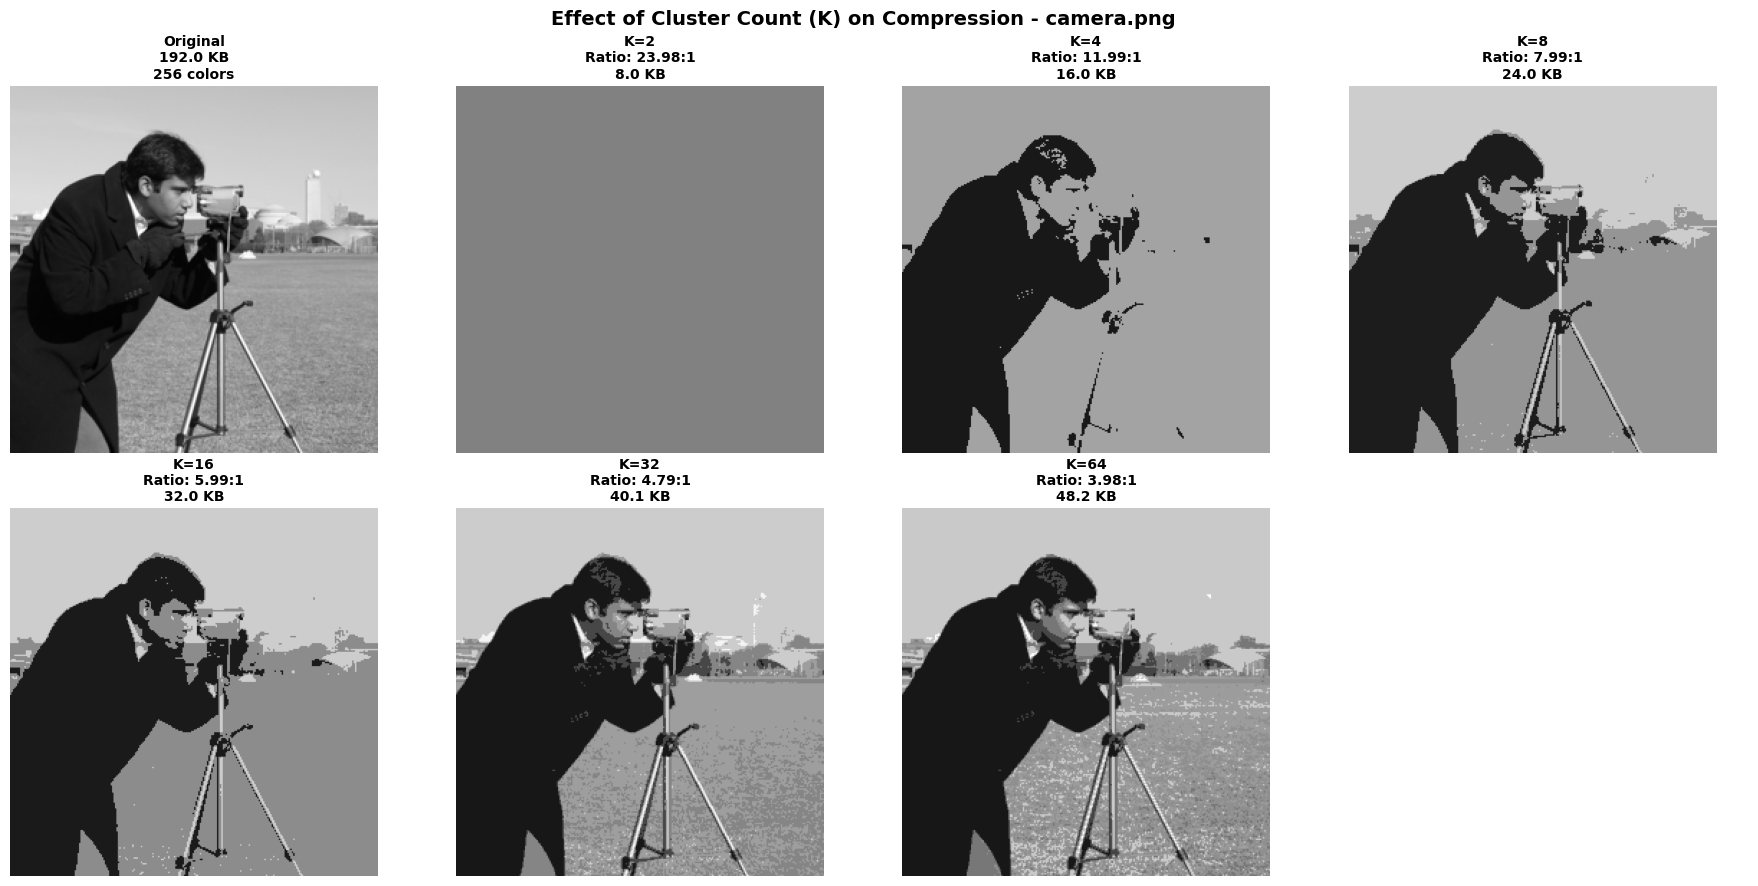
\includegraphics[width=0.8\textwidth]{gath_camera_effect.png}
    \caption{Original Cameraman image ($256\times256$).}
    \label{fig:gg_camera_original}
\end{figure}

\begin{figure}[H]
    \centering
    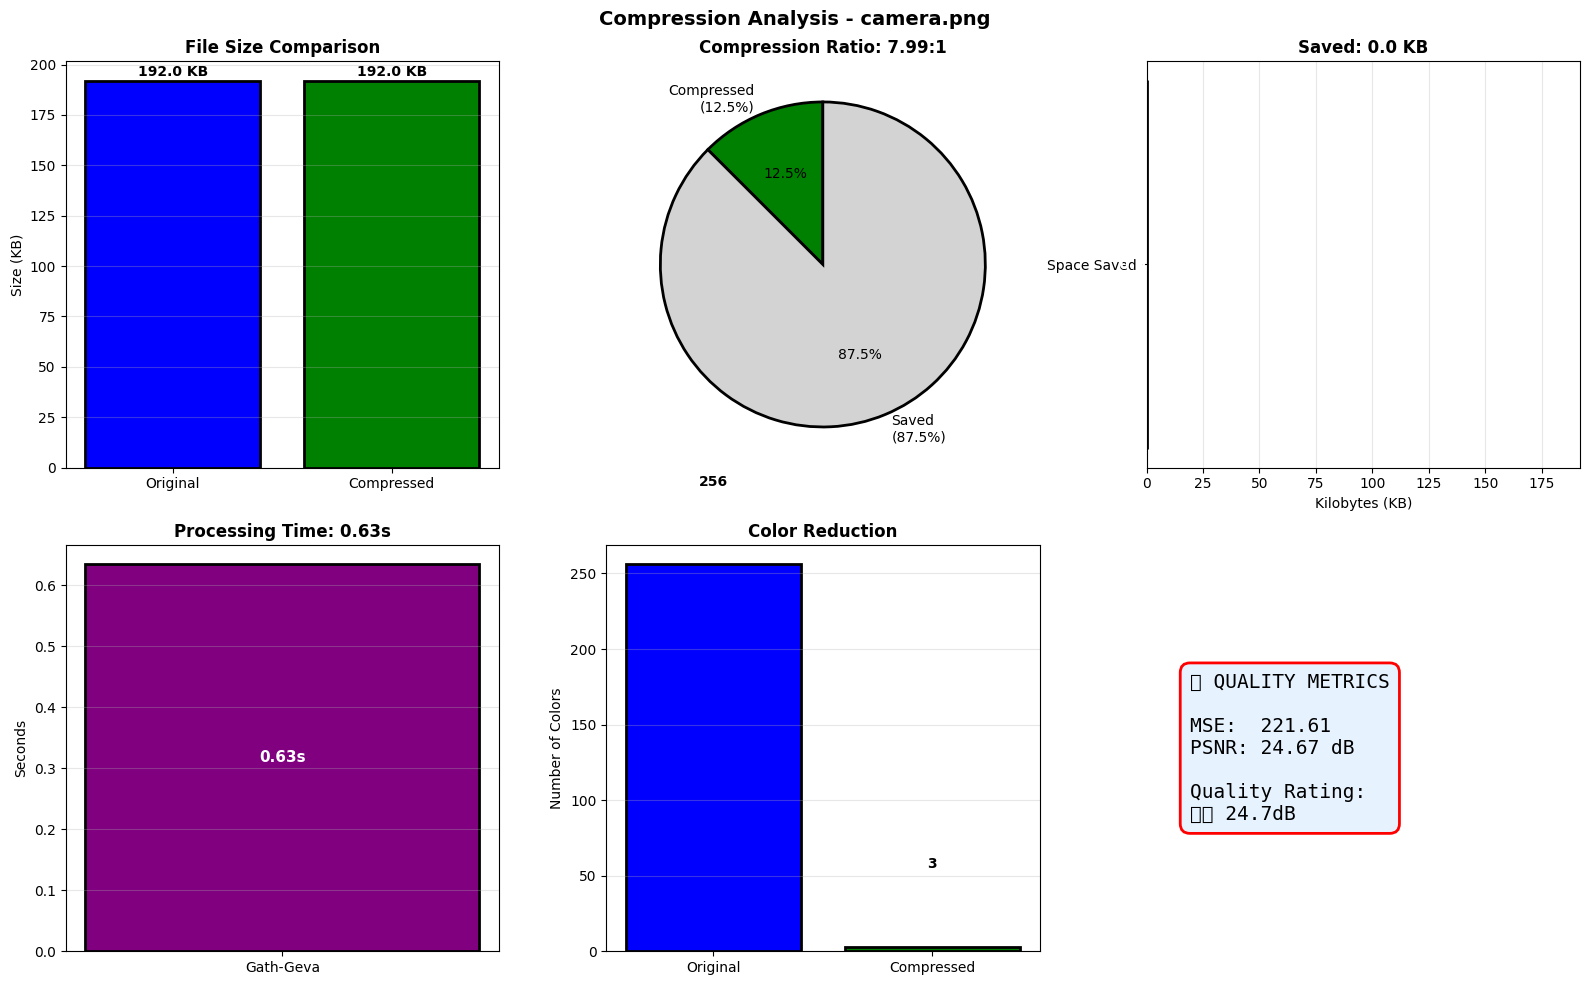
\includegraphics[width=0.8\textwidth]{gath_camera_chart.png}
    \caption{Cameraman image after Gath‑Geva clustering with $K=8$ clusters (vector quantisation).}
    \label{fig:gg_camera_clustered}
\end{figure}

\begin{figure}[H]
    \centering
    \includegraphics[width=0.8\textwidth]{gath_camera_clust.png}
    \caption{Residual image (original minus clustered). Dark areas indicate small errors.}
    \label{fig:gg_camera_residual}
\end{figure}




Figure~\ref{fig:gg_membership_example} visualises the fuzzy membership maps for a few selected clusters. Brighter regions indicate higher membership. Figure~\ref{fig:gg_compression_analysis} plots the compression ratio versus the number of clusters, showing diminishing returns beyond $K=8$. Finally, Figure~\ref{fig:gg_side_by_side} provides a side‑by‑side comparison of the original and reconstructed images for different $K$ values.

\begin{figure}[H]
    \centering
    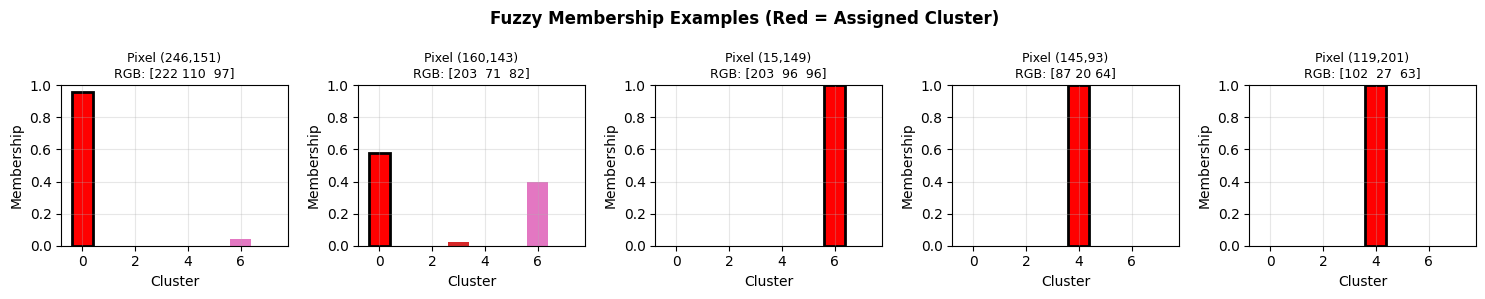
\includegraphics[width=1.0\textwidth]{gath_fuzzy_leena.png}
    \caption{Fuzzy membership maps for selected clusters (brighter = higher membership).}
    \label{fig:gg_membership_example}
\end{figure}

\begin{figure}[H]
    \centering
    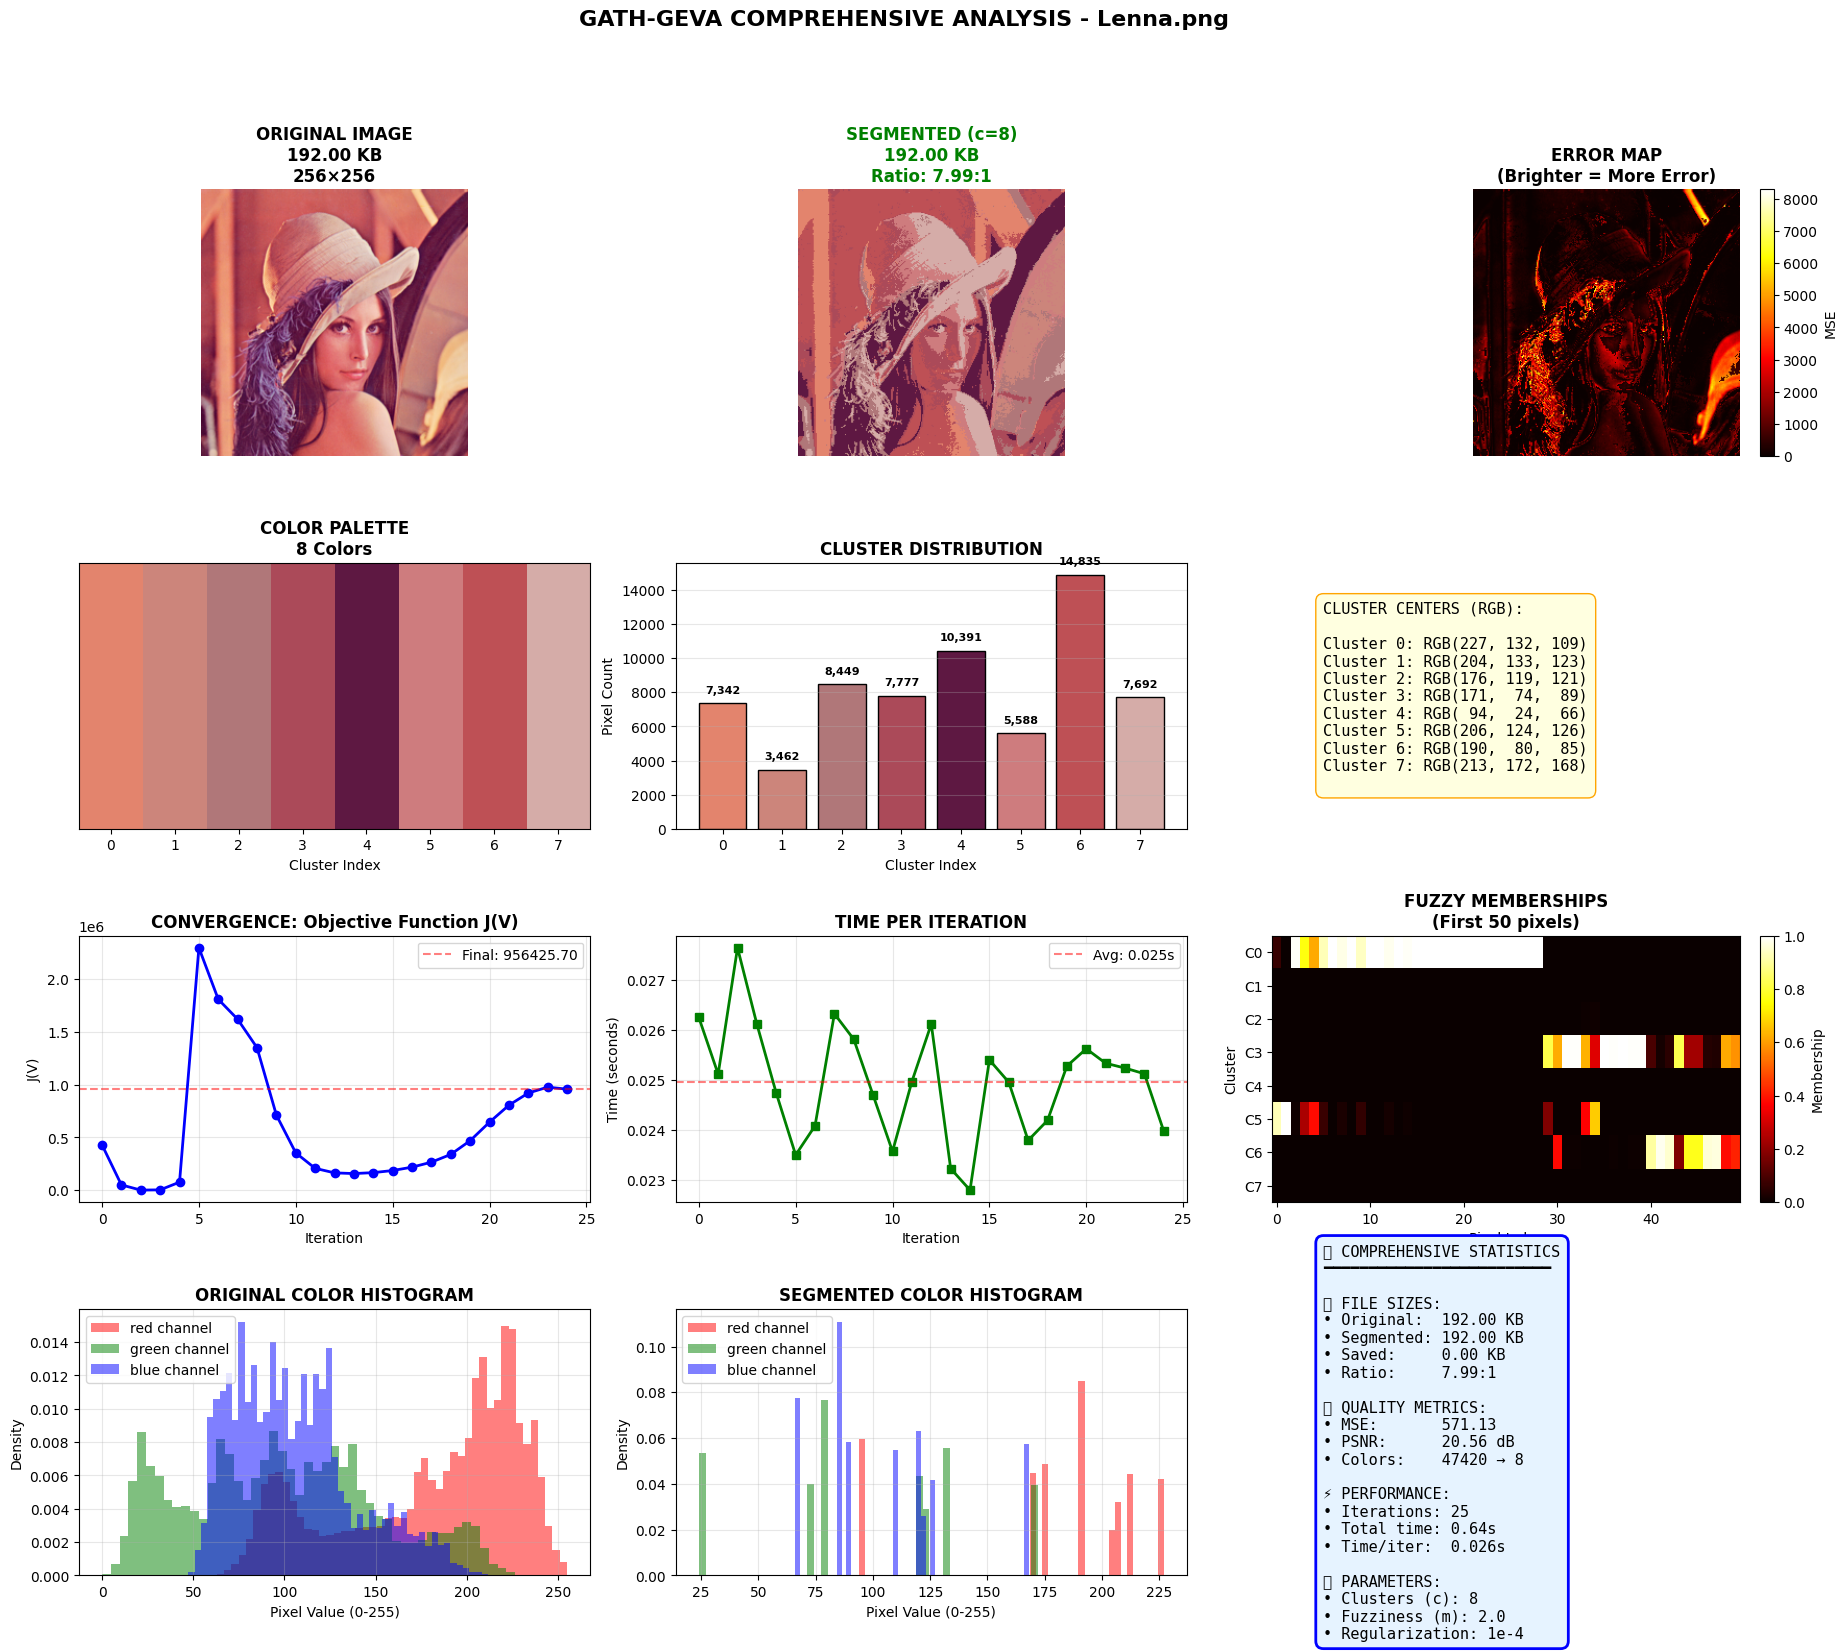
\includegraphics[width=1.0\textwidth]{gath_compare_leena.png}
    \caption{Compression ratio vs. number of clusters. The gain saturates after $K=8$.}
    \label{fig:gg_compression_analysis}
\end{figure}

\begin{figure}[H]
    \centering
    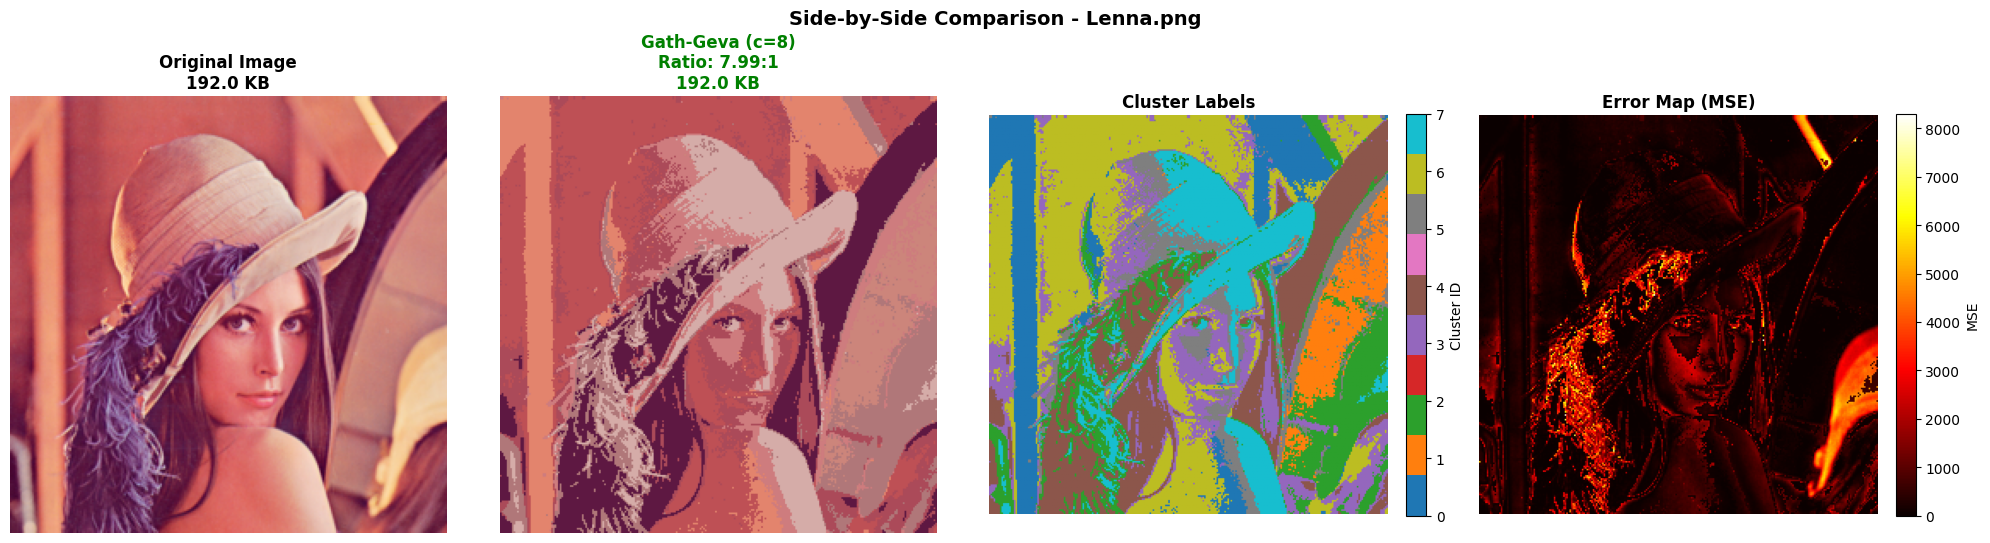
\includegraphics[width=1.0\textwidth]{gath_sidebyside_leena.png}
    \caption{Side‑by‑side comparison: original (left) and reconstructed with $K=8$ (right).}
    \label{fig:gg_side_by_side}
\end{figure}




\begin{figure}[H]
    \centering
    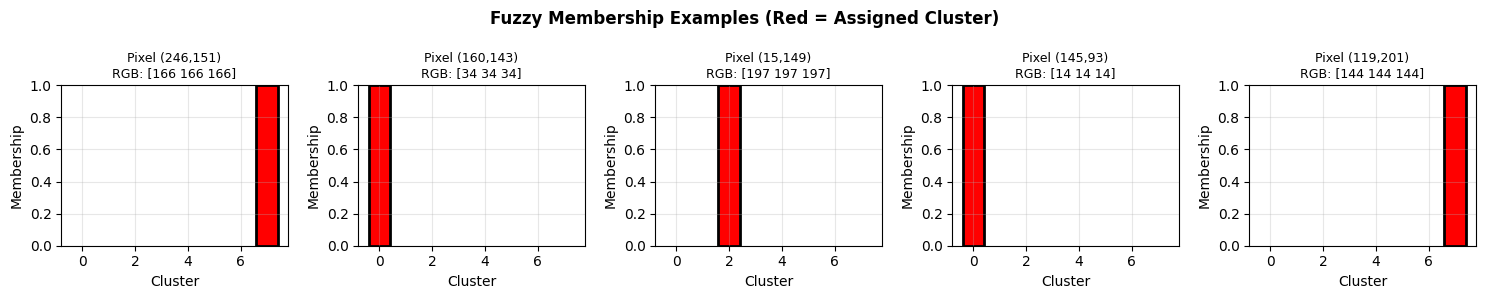
\includegraphics[width=1.0\textwidth]{gath_camera_fuzzy.png}
    \caption{Fuzzy membership maps for selected clusters (brighter = higher membership).}
    \label{fig:gg_membership_example_camera}
\end{figure}

\begin{figure}[H]
    \centering
    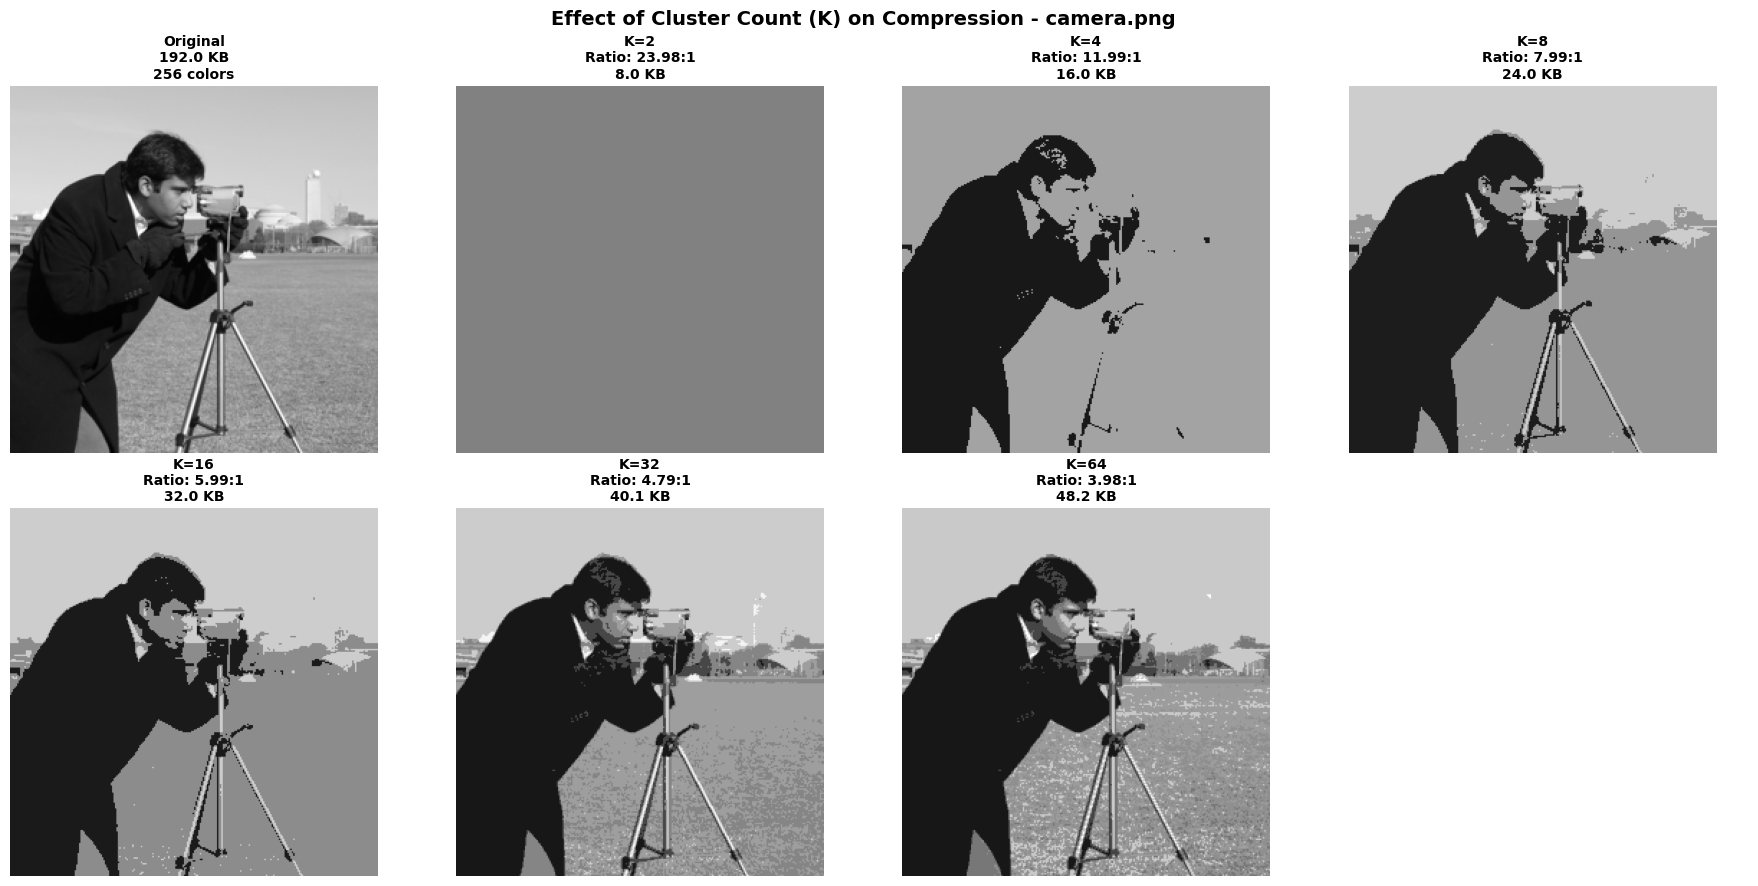
\includegraphics[width=1.0\textwidth]{gath_camera_effect.png}
    \caption{Compression ratio vs. number of clusters. The gain saturates after $K=8$.}
    \label{fig:gg_compression_analysis_camera}
\end{figure}

\begin{figure}[H]
    \centering
    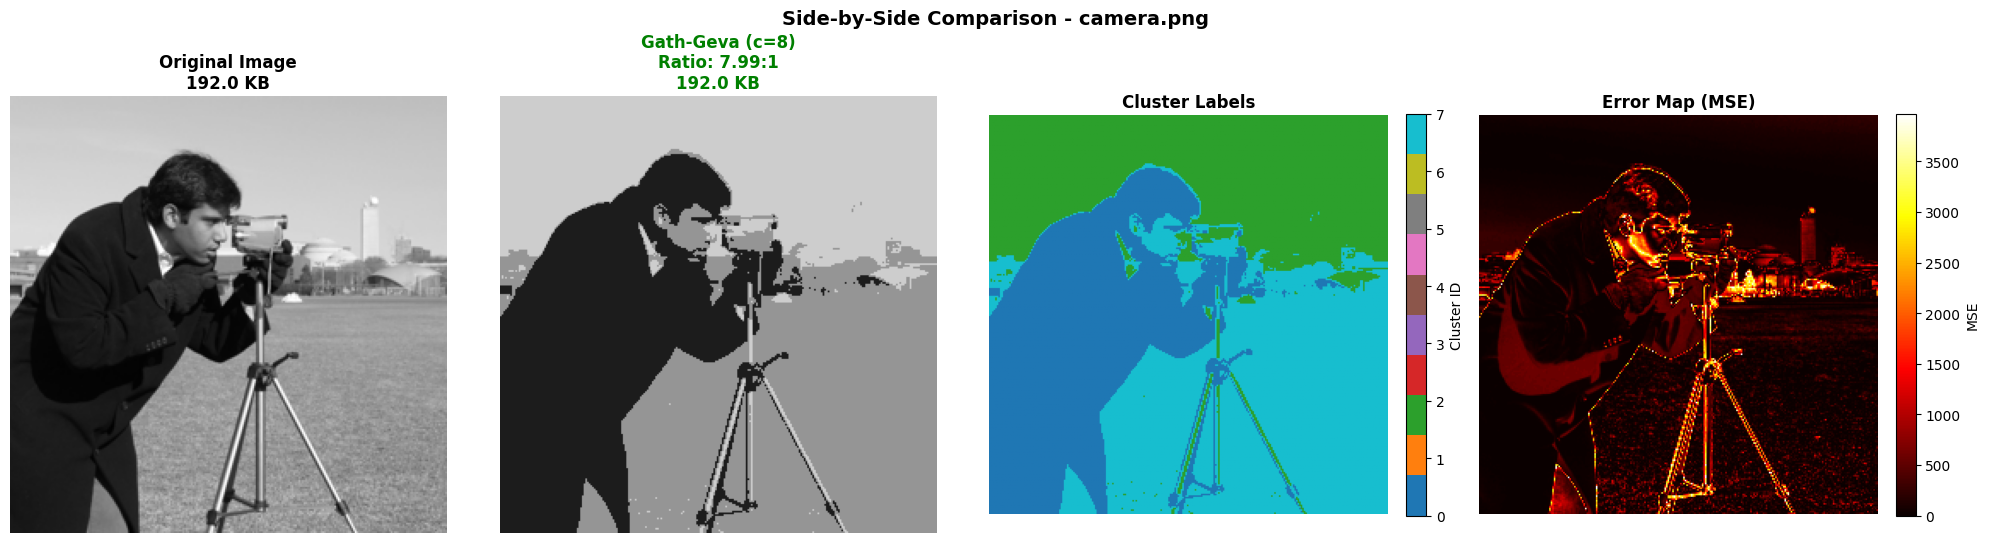
\includegraphics[width=1.0\textwidth]{gath_camera_sidebyside.png}
    \caption{Side‑by‑side comparison: original (left) and reconstructed with $K=8$ (right).}
    \label{fig:gg_side_by_side_camera}
\end{figure}





\paragraph{Discussion and Limitations}
\begin{itemize}
    \item \textbf{Advantages:} Gath‑Geva can model ellipsoidal clusters of varying sizes and densities, making it more flexible than spherical‑only algorithms. It provides fuzzy memberships that capture uncertainty.
    \item \textbf{Limitations:} The algorithm is computationally more expensive than K‑Means or FCM, especially for large datasets and high numbers of clusters. The need to compute and invert covariance matrices for each cluster at every iteration dominates the runtime.
    \item \textbf{Application to compression:} The compression ratio improves with more clusters (finer colour palette), but at the cost of higher computational time and diminishing perceptual returns. For $K=8$, the ratio $7.99:1$ is already excellent for lossy image compression.
\end{itemize}

\paragraph{Summary}
Gath‑Geva fuzzy clustering is a powerful unsupervised learning algorithm that can detect ellipsoidal clusters with different sizes and densities. Its mathematical formulation based on fuzzy membership, covariance matrices, and an exponential distance measure allows it to adapt to complex data distributions. Applied to image compression, it achieved a compression ratio of nearly $8:1$ on the Lenna image with only 8 clusters, demonstrating its effectiveness for vector quantisation. The algorithm’s time complexity scales approximately linearly with the number of clusters, making it suitable for moderate‑sized datasets. Future work could explore adaptive determination of the optimal number of clusters and integration with entropy coding for even higher compression gains.

\end{document}